%!TEX root = main.tex

\section{Application: Arithmetics autograder}
In the application of arithmetics autograder, the input image is ususally very large (typically around \(3000\times2000\) pixels), among which 10\% are black pixels.
This means if we apply ``Algorithm 4'' directly, the input list of coordinates typically have length \(10^5\) to \(10^6\), which is too long for the algorithm to return the results in reasonable period of time.
A more promising approach is to split the procedure into the following steps:
\begin{enumerate}
    \item cluster the worksheet into equations
    \item cluster the numbers and operators in each equation from step 1.
    \item handwritten recognition
\end{enumerate}

\subsection{Equation clustering}
One observation is that step 1 does not need accuracy in the numbers and operators, so that we can resample the input image so that the input for Algorithm 4 is significantly reduced (to around \(10^3\) coordinates of black pixels). We can see from \autoref{fig10b} is blurred compared with the input \autoref{fig10a}, and most of the equations are correctly clustered.
\begin{figure}[htbp]
    \vspace{-1em}
    \centering
    \begin{subfigure}[t]{0.8\textwidth}
        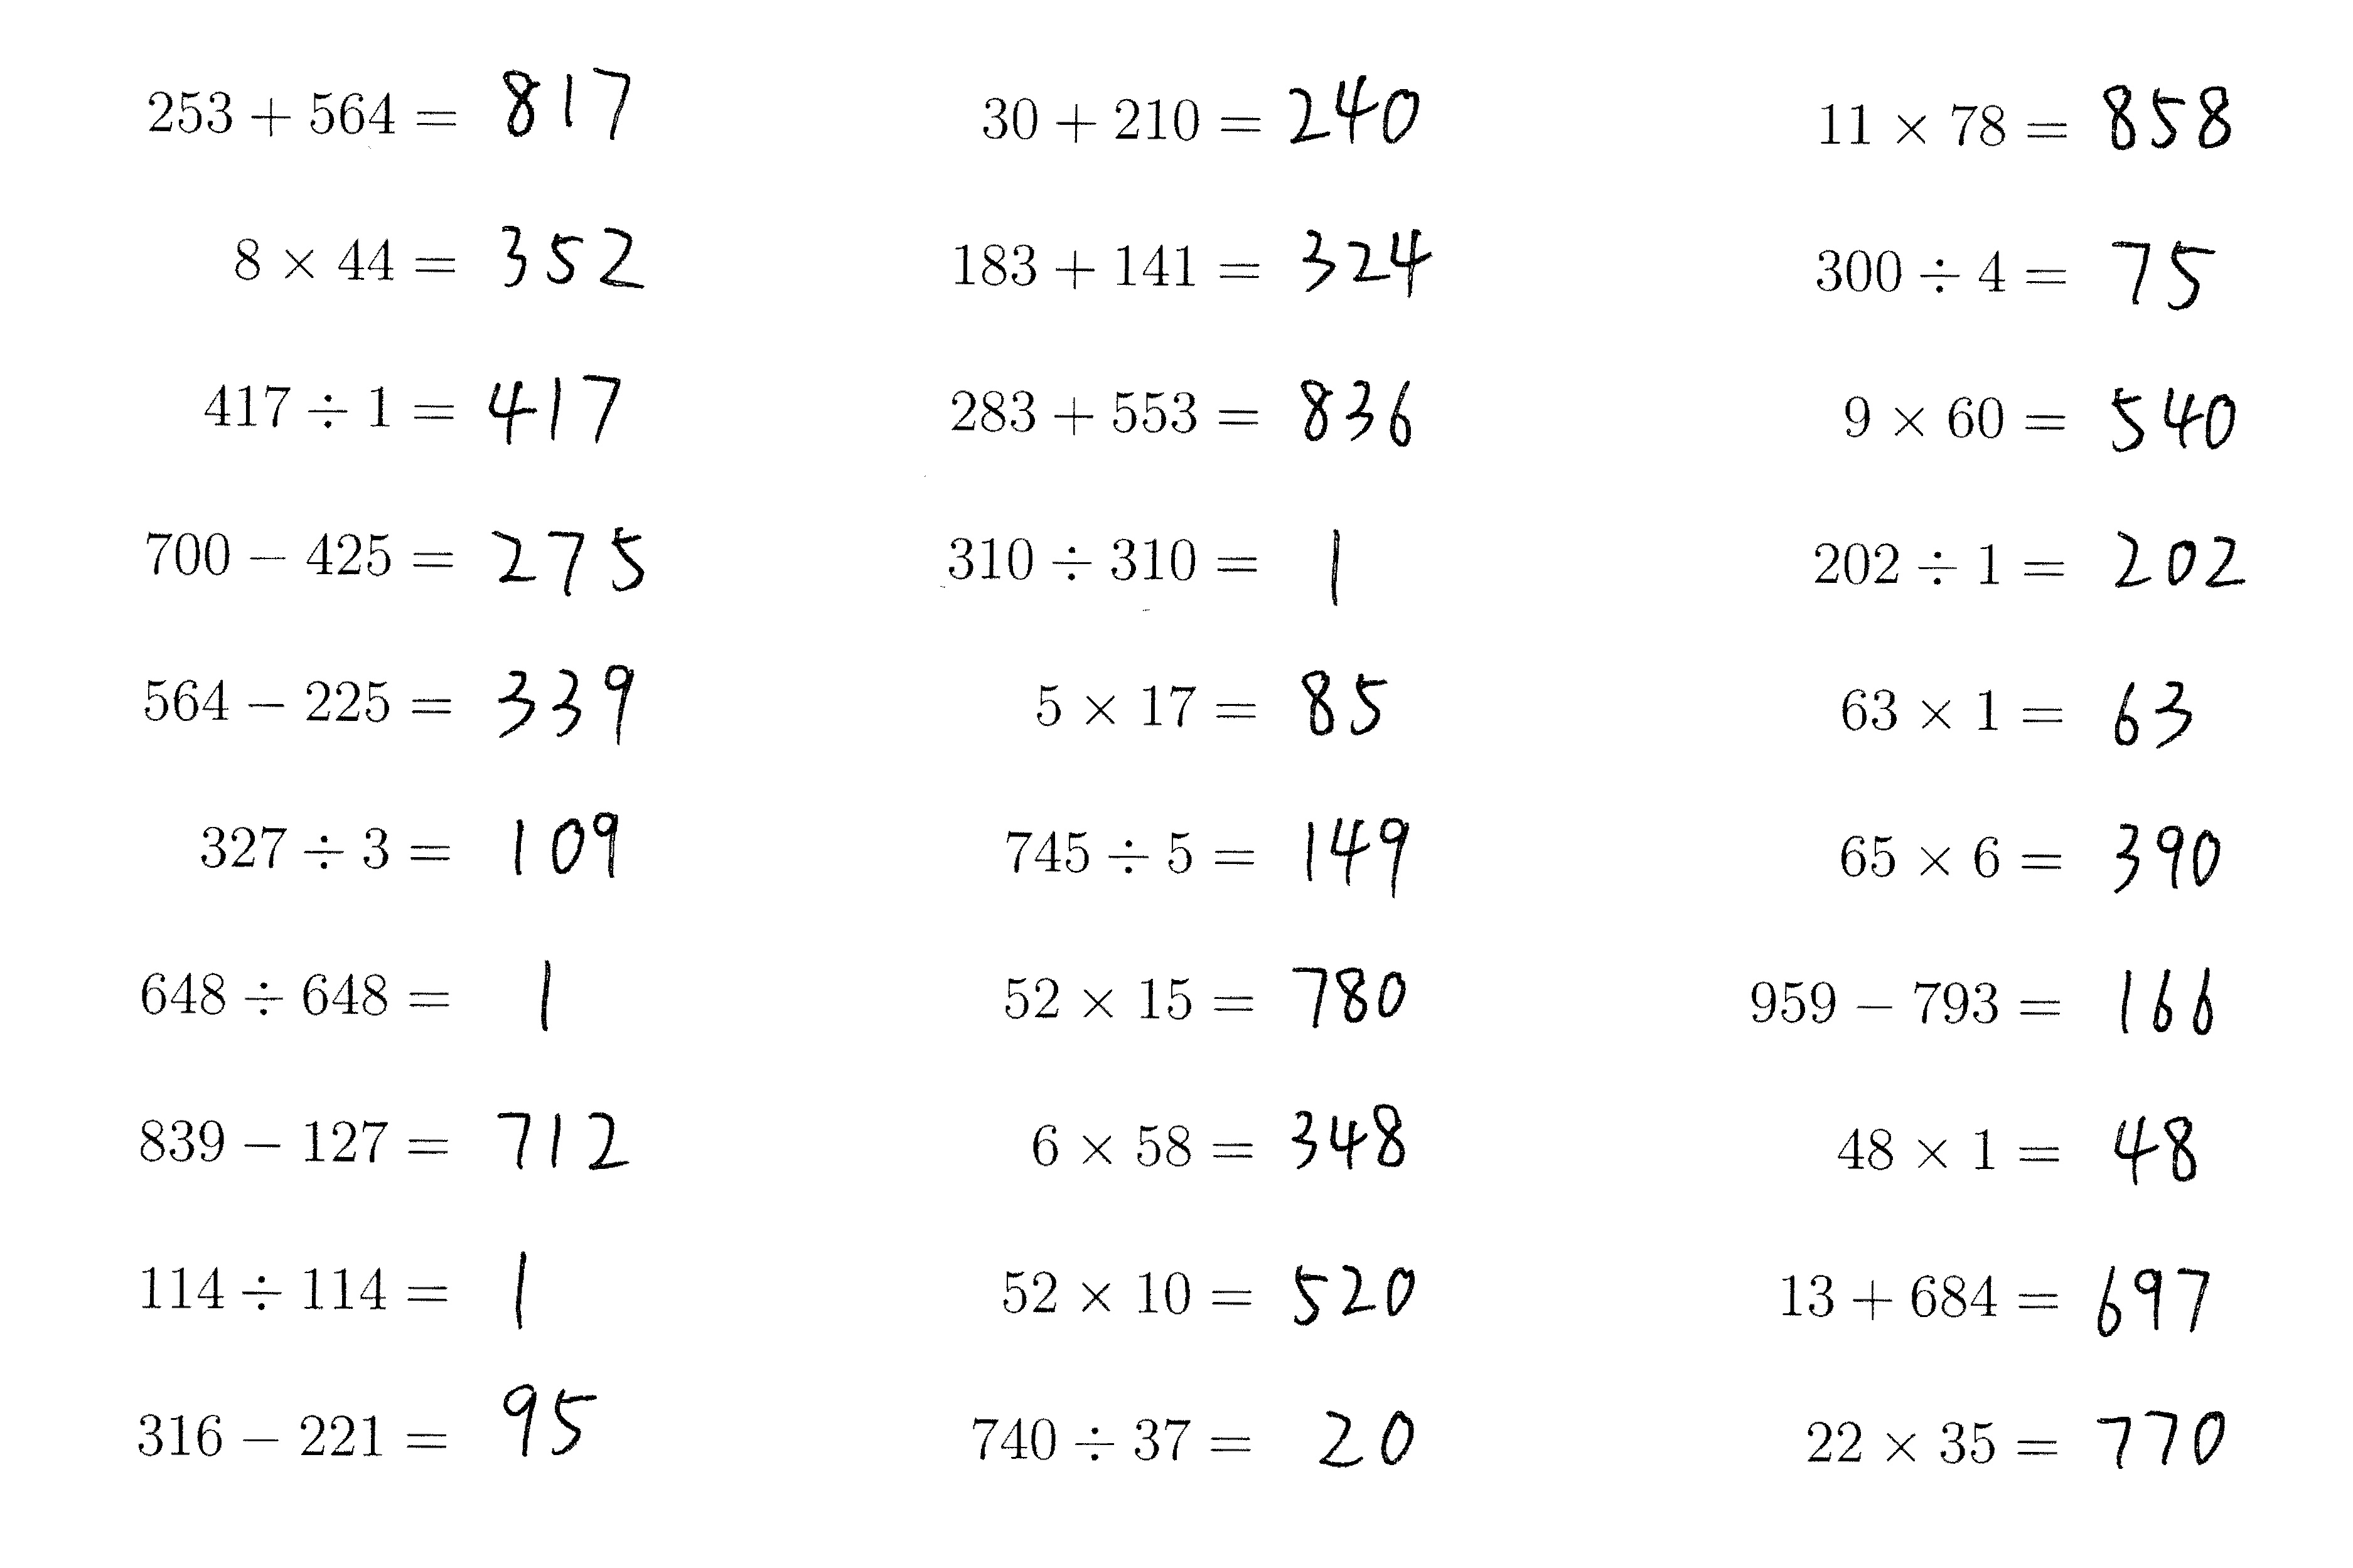
\includegraphics[width=\textwidth]{../TestSamplePictures/test1.png}
        \caption{Input image}\label{fig10a}		
    \end{subfigure}
    \begin{subfigure}[t]{0.8\textwidth}
        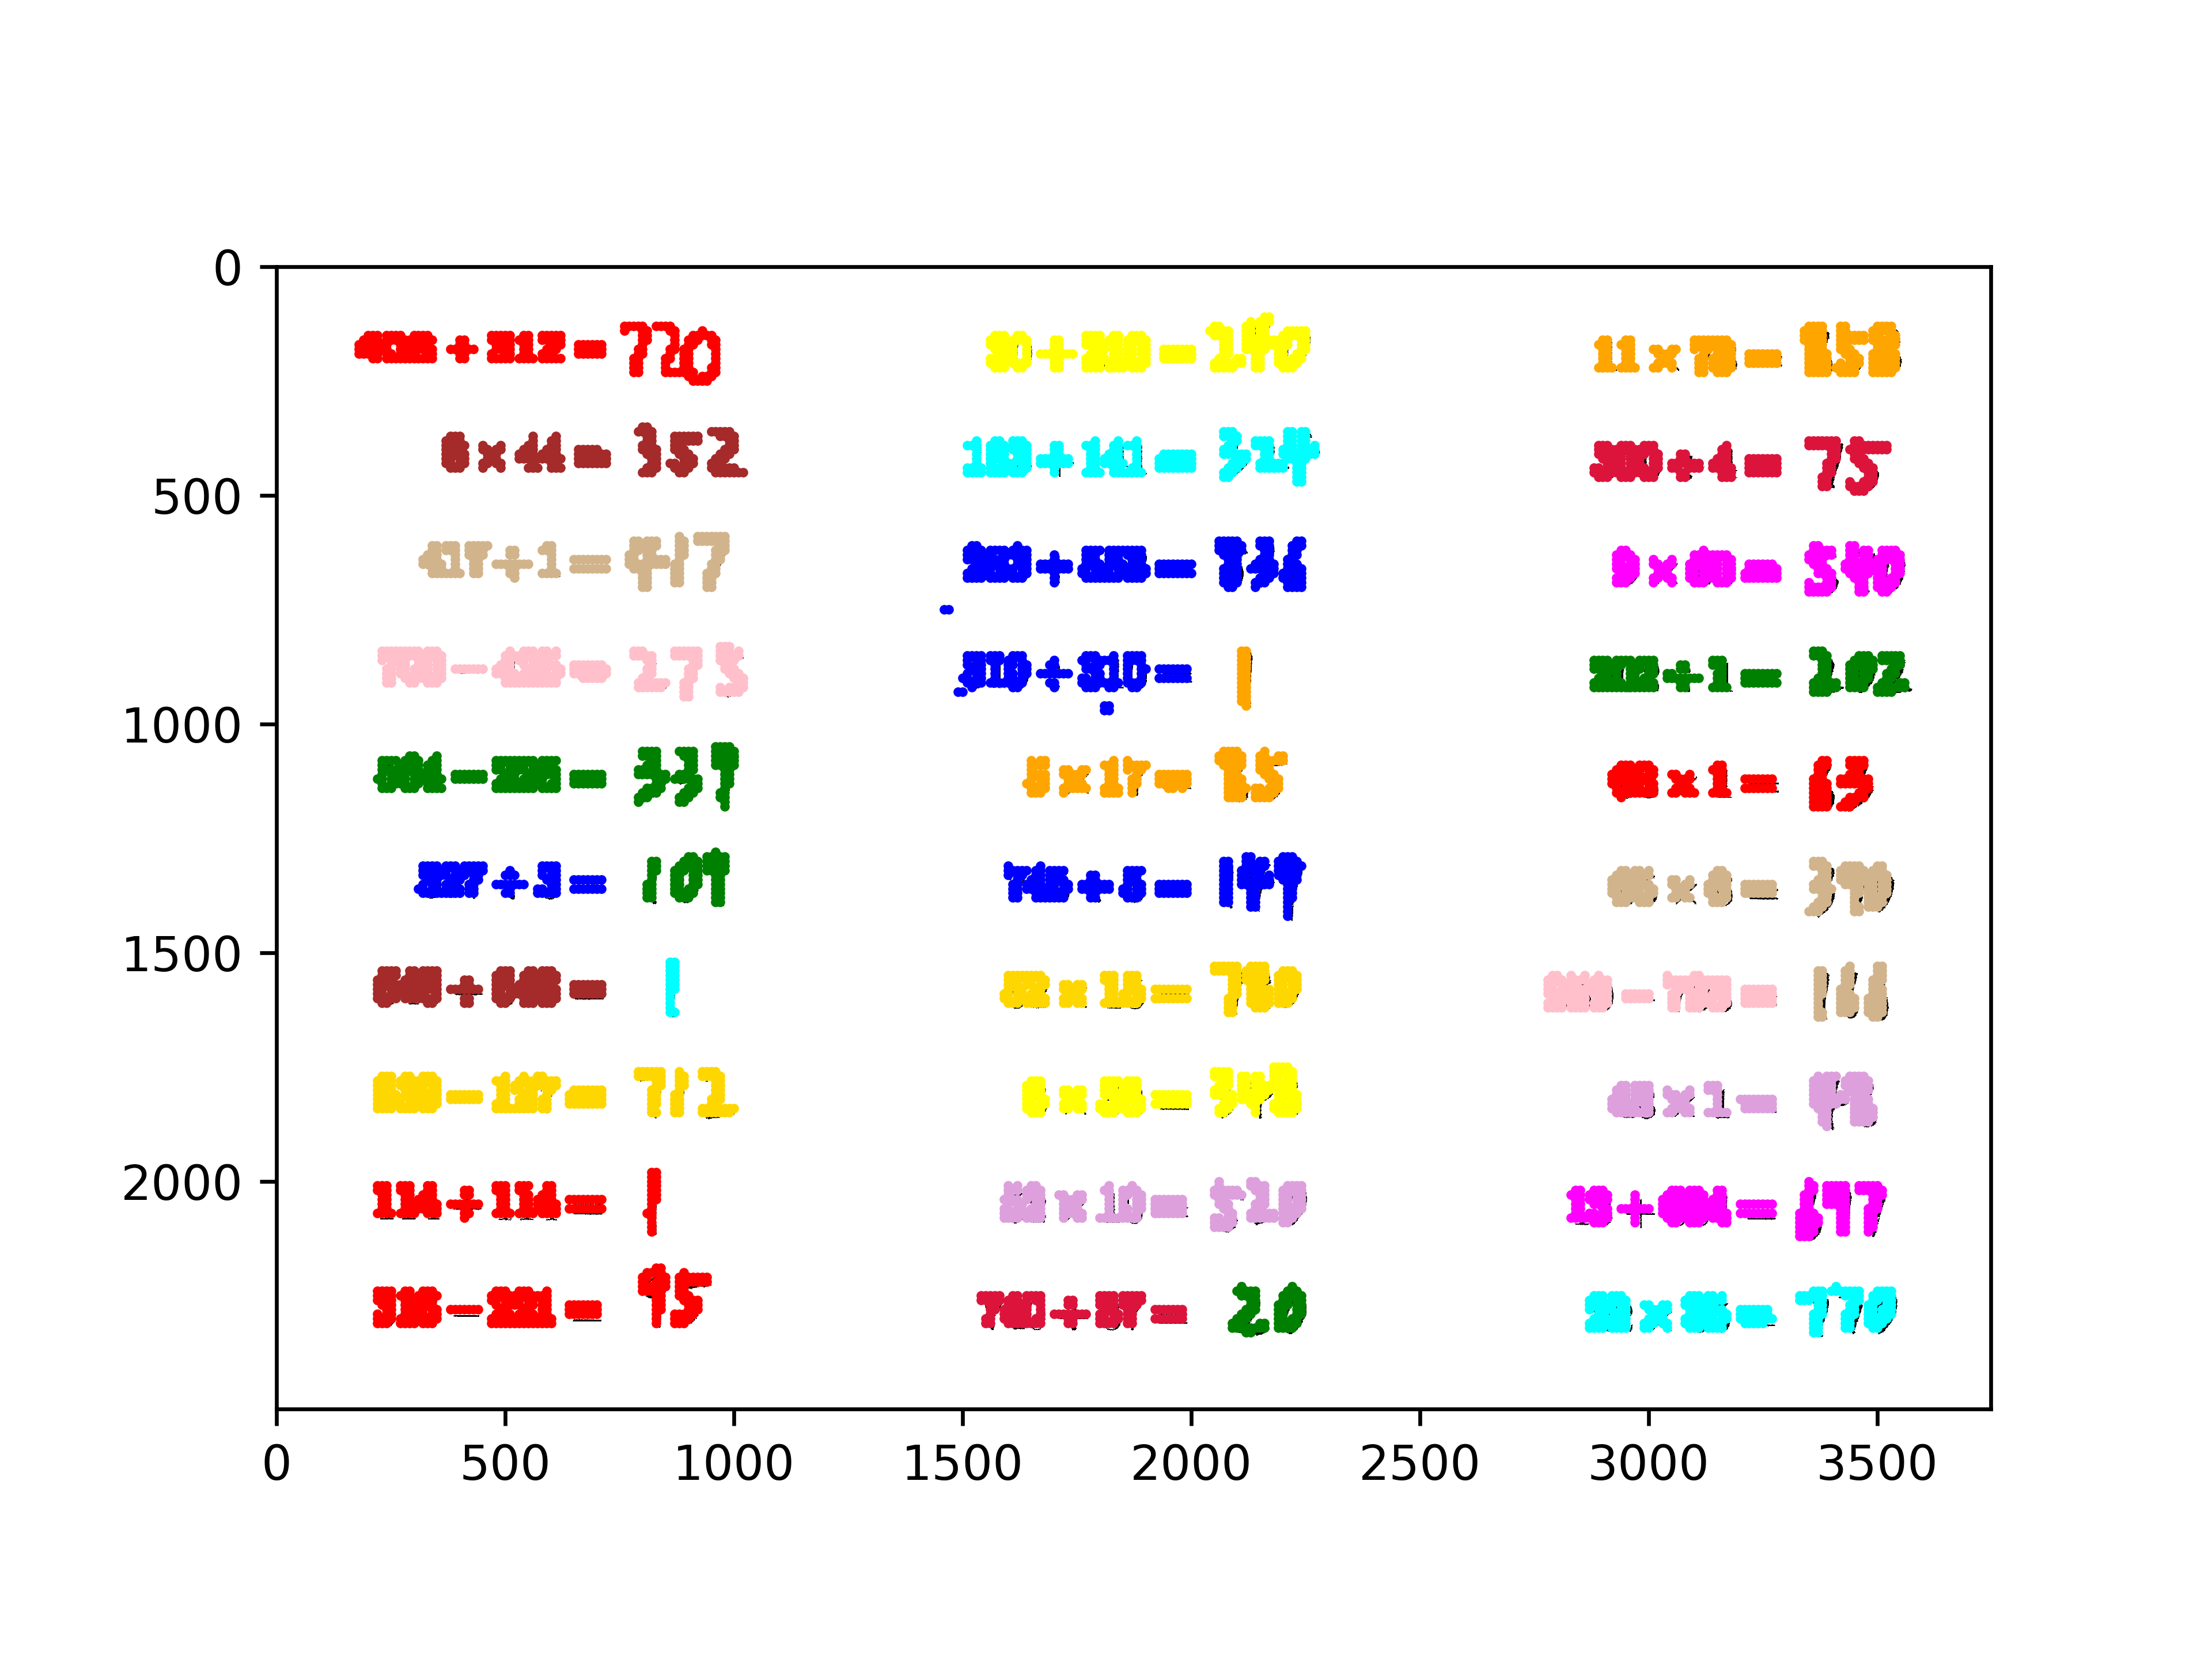
\includegraphics[width=\textwidth]{../TestSamplePictures/test_result.png}
        \caption{Equation clustering effect}\label{fig10b}
    \end{subfigure}
    \caption{Equation clustering by Algorithm 4}\label{fig10}
\end{figure}

\subsection{Numbers and operators clustering}
We take the first equation ``408 + 312 = 720" as an example and apply Algorithm 4 again.
The main goal in this section is to divide the equation into separete digits and symbols. Especially we deal with the intersection between handwritten ``2" and handwritten ``0". See \autoref{fig10}.

\begin{figure}[htbp]
    \vspace{-1em}
    \centering
    \begin{subfigure}[t]{1.2\textwidth}
	\hspace{-4em}
        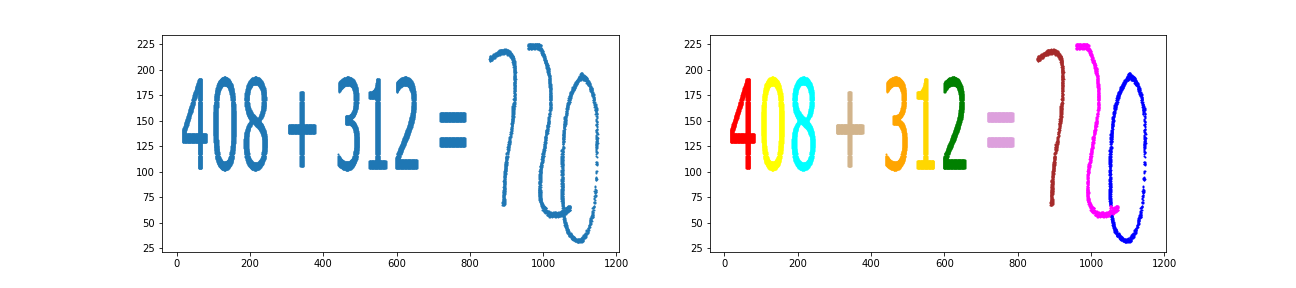
\includegraphics[width=\textwidth]{720_formula_output_1.png}
    \end{subfigure}
    \caption{Equation clustering by Algorithm 4}\label{fig10}
\end{figure}

\subsection{Handwritten recognition}
We implement handwritten recognition by using PCA. 
The results shows that we successfully recognize handwritten ``7" and ``2" but failed in handwritten ``0". 
However, it quite depends on the database we use, MNIST.
Handwritten digit recognition is a well-studied problem. Readers can use existing packages from open platform to handle this problem.
Since this is an irrelevant problem of our main project, we leave it as a future work.
